\labeledsection{STRIPS Planning}{sec:strips}
\definition{STRIPS}{
The Stanford Research Institute Problem Solver (STRIPS) is a formal planning language that represents states and actions using \linkterm{propositional logic}{def:pl0_as_ls}.
}{strips}

\commandnote{
\begin{itemize}
    \item \linkterm{STRIPS}{strips} utilizes \linkterm{propositional}{def:pl0_as_ls} variables as \linkterm{atomic formulae}{atomic_formula} to define world states.
    \item \textbf{Preconditions:} A conjunction of \linkterm{atoms}{atomic_formula} that must be satisfied to execute an action.
    \item \textbf{Effects:} A conjunction of \linkterm{literals}{literal} (additions and deletions) specifying how the state is modified by an action.
    \item \textbf{Goals:} A conjunction of \linkterm{atoms}{atomic_formula} defining the conditions required for a problem to be considered solved.
\end{itemize}
}

\definition{STRIPS Task}{
A \textbf{STRIPS Task} is a quadruple $\tuple{\mathcal{F}, \mathcal{A}, \mathcal{I}, \mathcal{G}}$ where:
\begin{itemize}
\item $\mathcal{F}$ is a \linkterm{finite}{set_cardinality} \linkterm{set}{def:set} of \textbf{facts} which are \linkterm{atomic}{atomic_formula} \linkterm{propositions}{proposition} in \linkterm{$\text{PL}^0$}{def:pl0_as_ls} or \linkterm{$\text{PL}^\text{nq}$}{plnq}. E.g. $\text{clean}(\text{room}), \text{robot\_at}(\text{door})$
\item $\mathcal{A}$ is a \linkterm{finite}{set_cardinality} \linkterm{set}{def:set} of \textbf{actions}.
\item An action $a \in \mathcal{A}$ is a triple $a:=\tuple{\text{pre}_a, \text{add}_a, \text{del}_a}$ of \linkterm{subsets}{subset} of $\mathcal{F}$.
\begin{itemize}
    \item $\text{pre}_a$ are the \textbf{preconditions} of $a$
    \item $\text{add}_a$ is a list of facts that become true when $a$ is successfully applied
    \item $\text{del}_a$ is a list of facts that must be deleted after applying $a$
\end{itemize}
For example, we represent action $\text{drive}(x,y)$ as $\tuple{\set{\text{at}(x)}, \set{\text{at}(y), \text{visited}(y)}, \set{\text{at}(x)}}$
\item $\mathcal{I} \subseteq \mathcal{F}$ is the initial state (facts that are true initially), e.g. initially we are at Sydney $\leadsto \set{\text{at}(\text{Sy}), \text{visited}(\text{Sy})}$
\item $\mathcal{G \subseteq \mathcal{F}}$ is the goal state, e.g. \textit{agent must start from Sydney, visit all cities, then go back to Sydney} $\leadsto \set{\text{at}(\text{Sy})} \cup \set{\text{visited}(x) \mid x \in \set{\text{Sy}, \text{Ad}, \text{Br}, \text{Pe}, \text{Da}}}$
\end{itemize}
}{strips_task}

\definition{STRIPS Task Solution}{
A solution to a \linkterm{STRIPS task}{strips_task} is called a \text{plan}
}{strips_plan}

\definition{STRIPS as Search}{
A \linkterm{plan}{strips_plan} for a \linkterm{STRIPS task}{strips_task} $\Pi := \tuple{\mathcal{F}, \mathcal{A}, \mathcal{I}, \mathcal{G}}$ is a \linkterm{solution}{search_prob_sol} to an induced \linkterm{search problem}{search_problem} $\Theta_{\Pi} := \tuple{\mathcal{S}_{\Pi}, \mathcal{A}_{\Pi}, \mathcal{T}_{\Pi}, \mathcal{I}_{\Pi}, \mathcal{G}_{\Pi}}$, where:
\begin{itemize}
    \item $\mathcal{S}_{\Pi} := \powerset{\mathcal{F}}$ is the \linkterm{set}{def:set} of all possible states
    \item $\mathcal{A}_{\Pi} := \mathcal{A}$
    \item $\mathcal{I}_{\Pi} := \mathcal{I}$
    \item $\mathcal{G}_{\Pi} := \{s \in \mathcal{S}_{\Pi} \mid \mathcal{G} \subseteq s\}$ (Goal satisfaction via set inclusion)
    \item $\func{\mathcal{T}_{\Pi}}{\cartprod{\mathcal{A}_{\Pi}, \mathcal{S}_{\Pi}}}{\powerset{\mathcal{S}_{\Pi}}}$ is the transition model defined as:
    \[
    \mathcal{T}_{\Pi}(a, s) = \begin{cases} 
    \{(s \setminus \text{del}_a) \cup \text{add}_a\} & \text{if } \text{pre}_a \subseteq s \\
    \emptyset & \text{otherwise}
    \end{cases}
    \]
\end{itemize}
}{strips_as_search}

\definition{Partially Ordered Plan (POP)}{
Let $\Pi := \tuple{\mathcal{F}, \mathcal{A}, \mathcal{I}, \mathcal{G}}$ be a \linkterm{STRIPS task}{strips_task}, then a \textbf{partially ordered plan} $P := \tuple{V,E}$ is a \linkterm{labeled}{labeled_graph} \linkterm{DAG}{dag} where the \linkterm{nodes}{directed_graph} in $V$ are the steps (actions), where we have two special steps:
\begin{itemize}
\item \textbf{start}: This is the step that has no preconditions and its effects are simply $\mathcal{I}$
\item \textbf{finish}: This is the step that has no effects and its preconditions are simply $\mathcal{G}$
\end{itemize}
An edge $e := \tuple{S,T} \in E$ defines the relation between steps. We have two types of constrainst:
\begin{itemize}
    \item \textbf{causal links}: Written as $S \xrightarrow{p} T$. It means step $S$ is performed to achieve fact $p$ because step $T$ needs $p$ to be true (precondition of $T$)
    \item \textbf{temporal constraints}: Written as $S \prec T$. It means $S$ must happen before $T$
\end{itemize}
Additionally, we define an \textbf{open condition} to represent a \textit{missing link}. If a step $T$ has precondition $p$, but no causal link $S \xrightarrow{p} T$ exists yet, the plan is incomplete.
}{pop_strips}

\definition{Possibly Intervening}{
Let $P$ be a \linkterm{partially ordered plan}{pop_strips}, then we call a step $U$ \textbf{possibly intervening} in a causal link $S \xrightarrow{p} T$, iff $P \cup \set{S \prec U, U \prec T}$ is \linkterm{acyclic}{cyclic_graphs}. 
}{possibly_intervening}

\definition{Achieved Precondition}{
A precondition is \textbf{achieved} iff it is the effect of an earlier step and no \linkterm{possibly intervening step}{possibly_intervening} undoes it. 
}{achieved_precondition}

\definition{Complete Plan}{
A \linkterm{partially ordered plan}{pop_strips} is called \textbf{complete} iff every precondition of every step is \linkterm{achieved}{achieved_precondition}.
}{complete_plan}

\definition{Partial Order Planning}{
The process of computing \linkterm{complete}{complete_plan} and \linkterm{acyclic}{cyclic_graphs} \linkterm{partially ordered plans}{pop_strips} for a given planning task.
}{partial_order_planning}

\commandnote{
\begin{minipage}[c]{0.7\textwidth}
In diagrams, we often write \linkterm{STRIPS}{strips} actions into boxes with preconditions above and effects below.
\end{minipage}
\hfill
\begin{minipage}[c]{0.2\textwidth}
\begin{tikzpicture}
    \node[draw, thick, minimum width=2.5cm, minimum height=0.8cm] (buy) {buy(x)};
    \node[above=0.1cm of buy, font=\footnotesize] {at(p), sells(p,x)};
    \node[below=0.1cm of buy, font=\footnotesize] {have(x)};
\end{tikzpicture}
\end{minipage}
}

\commandnote{
\begin{itemize}
    \item A causal link $S \xrightarrow{p} T$ can be represented by a direct arrow between the effects ($p$) of $S$ and the preconditions ($p$) of $T$
    \item Temporal constraints can be denoted via dashed arrows
\end{itemize}
}


\definition{Clobbering}{
In a \linkterm{partially ordered plan}{pop_strips}, a step $C$ \textbf{clobbers} a causal link $L := S \xrightarrow{p} T$, iff it destroys the condition $p$ achieved by $L$. We sometimes refer to $C$ as a \textbf{threat}.
}{clobbers}

\commandnote{
$C$ is a \linkterm{threat}{clobbers} if:
\begin{itemize}
    \item $C$ is \linkterm{possibly intervening}{possibly_intervening} in $S \xrightarrow{p} T$.
    \item $p \in \text{del}_C$ (the action $C$ deletes the required fact).
\end{itemize}
}

\definition{}{
If $C$ \linkterm{clobbers}{clobbers} $S \xrightarrow{p} T$ in a \linkterm{partially ordered plan}{pop_strips} $P$, then we can solve the conflict by either:
\begin{itemize}
    \item \textbf{demotion}: add a temporal constraint $C \prec S$ to $P$, or 
    \item \textbf{promotion}: add $T \prec C$ to $P$
\end{itemize}
}{demotion_promotion}

\commandnote{
Note that we should always make sure that we have an \linkterm{acyclic}{cyclic_graphs} graph. If our plan already has constraint $S \prec C$, then we cannot use \linkterm{demotion}{demotion_promotion} ($C \prec S$) because that would create $S \prec C \prec S$. Similarly, if the plan already has $C \prec T$, we cannot use \linkterm{promotion}{demotion_promotion} ($T \prec C$) because that would create $C \prec T \prec C$
}

\definition{Totally Ordered Plan}{
A \linkterm{partially ordered plan}{pop_strips} is \textbf{totally ordered} iff for every pair of distinct steps $S, T \in V$, either $S \prec T$ or $T \prec S$ is in the set of constraints.
}{totally_ordered}

\definition{Linearization}{
A \textbf{linearization} of a \linkterm{partially ordered plan}{pop_strips} $P$ is a \linkterm{totally ordered plan}{totally_ordered} that is consistent with all constraints in $P$.
}{linearization}

\commandnote{
A common point of confusion is equating a \linkterm{complete}{complete_plan} plan with a \linkterm{totally ordered}{totally_ordered} one. In  \linkterm{Partial Order Planning}{partial_order_planning}, these are distinct concepts:
\begin{itemize}
    \item \textbf{Completeness is about Logic:} A plan is complete when every "why" is answered (every precondition has a causal link) and every "conflict" is resolved (no \linkterm{threats}{clobbers}).
    \item \textbf{Total Ordering is about Time:} A plan is totally ordered only when every action is forced into a single sequence (a straight line).
\end{itemize}

A \linkterm{complete}{complete_plan} plan \textbf{might not} be \linkterm{totally ordered}{totally_ordered}. For example, if I need to "Buy Milk" and "Buy Bread" before I "Go Home," a complete plan will have causal links for both, but it won't care if I buy milk first or bread first. The actions remain "floating" relative to each other.

We only require a \linkterm{total ordering}{totally_ordered} (a \linkterm{linearization}{linearization}) at the moment of execution, but the planning process is finished as soon as the plan is \linkterm{complete}{complete_plan}.
}

\textbf{Example: }
Consider the following \linkterm{STRIPS task}{strips_task}:
\begin{itemize}
    \item We have three blocks $B := \set{A,B,C}$ and we have a table $T$.
    \item Fact: $\text{on}(X,Y)$ for $X \in B$ and $Y \in B \cup T$ to say that one block is on top of the other or is it at the table
    \item Fact: $\text{cl}(X)$ to say that nothing is on top of $X$
    \item Initial state: $C$ is clear and on top of $A$ which is on top of table. $B$ is clear and on top of table
    \item Goal state: $A$ is clear and on top of $B$ which is on top of $C$ which is on top of table 
    \item Action: $\text{move}(X,Y)$ to move $X$ to be on top of $Y$ ($X,Y \in B$)
    \begin{itemize}
        \item Pre: $\text{cl}(Y), \text{cl}(X), \text{on}(X,Z) \quad Z \in B \cup T$
        \item Add: $\text{cl}(Z) (\text{if }Z \neq T), \text{on}(X,Y)$
        \item Del: $\text{cl}(Y), \text{on}(X,Z)$
    \end{itemize}
    \item Action: $\text{move}(X,T)$ to move $X$ to be on top of $T$
    \begin{itemize}
        \item Pre: $\text{cl}(X), \text{on}(X,Y) \quad X,Y \in B$
        \item Add: $\text{cl}(Y), \text{on}(X,T)$
        \item Del: $\text{on}(X,Y)$
    \end{itemize}
\end{itemize}

Here is the \linkterm{totally ordered plan}{totally_ordered} to solve the problem:

\begin{figure}[H]
\centering

\begin{minipage}[c]{0.40\linewidth}
\centering
\includegraphics[width=\linewidth]{images/sussman.png}
\end{minipage}
\hfill
\begin{minipage}[c]{0.55\linewidth}
\centering
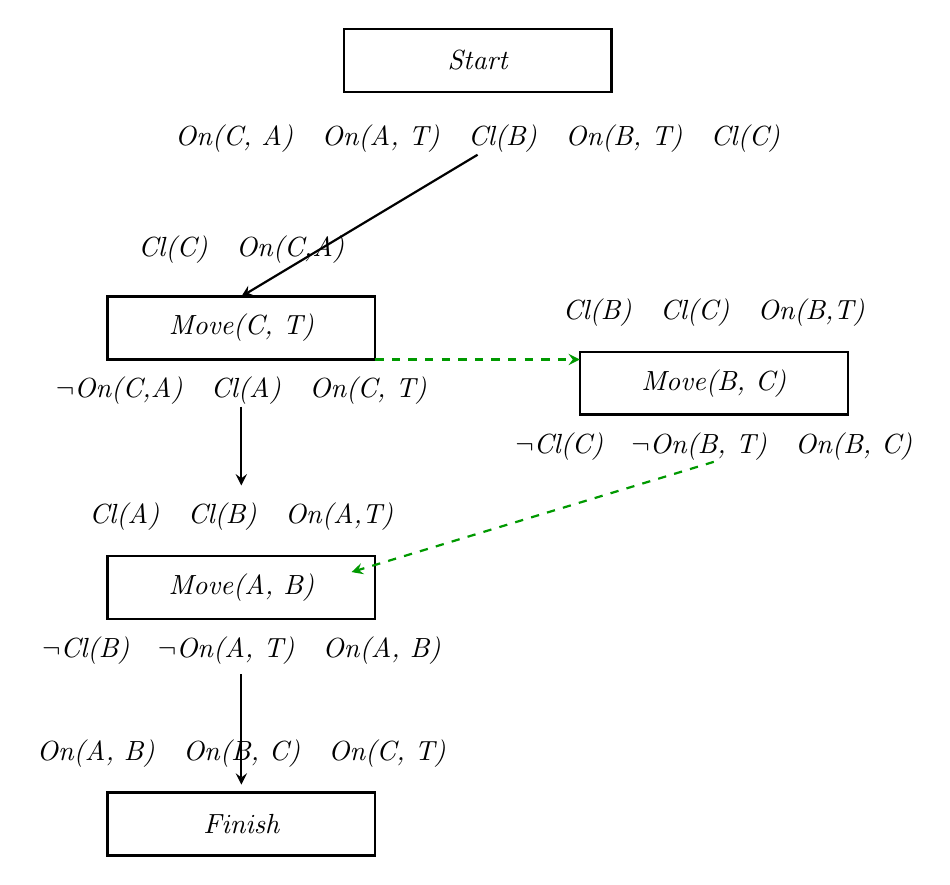
\begin{tikzpicture}[font=\itshape, >=stealth, thick]

\tikzset{
  action/.style={draw, rectangle, minimum width=34mm, minimum height=8mm, align=center},
  state/.style={align=center},
  darr/.style={->, dashed, green!60!black}
}

% Start
\node[action] (start) at (0,8) {Start};
\node[state] at (0,7) {On(C, A)\quad On(A, T)\quad Cl(B)\quad On(B, T)\quad Cl(C)};

% Move C T
\node[state]  at (-3,5.6) {Cl(C)\quad On(C,A)};
\node[action] (mCT) at (-3,4.6) {Move(C, T)};
\node[state]  at (-3,3.8) {$\neg$On(C,A)\quad Cl(A)\quad On(C, T)};

\draw[->] (0,6.8) -- (-3,5);

% Move B C
\node[state]  at (3,4.8) {Cl(B)\quad Cl(C)\quad On(B,T)};
\node[action] (mBC) at (3,3.9) {Move(B, C)};
\node[state]  at (3,3.1) {$\neg$Cl(C)\quad $\neg$On(B, T)\quad On(B, C)};

\draw[darr] (-1.3,4.2) -- (1.3,4.2);

% Move A B
\node[state]  at (-3,2.2) {Cl(A)\quad Cl(B)\quad On(A,T)};
\node[action] (mAB) at (-3,1.3) {Move(A, B)};
\node[state]  at (-3,0.5) {$\neg$Cl(B)\quad $\neg$On(A, T)\quad On(A, B)};

\draw[->] (-3,3.6) -- (-3,2.6);
\draw[darr] (3,2.9) -- (-1.6,1.5);

% Finish
\node[state]  at (-3,-0.8) {On(A, B)\quad On(B, C)\quad On(C, T)};
\node[action] (finish) at (-3,-1.7) {Finish};

\draw[->] (-3,0.2) -- (-3,-1.2);

\end{tikzpicture}
\end{minipage}

\end{figure}



\definition{Heuristic}{
Let $\Pi := \tuple{\mathcal{F}, \mathcal{A}, \mathcal{I}, \mathcal{G}}$ be a \linkterm{STRIPS task}{strips_task} and $\Theta_{\Pi} := \tuple{\mathcal{S}_{\Pi}, \mathcal{A}_{\Pi}, \mathcal{T}_{\Pi}, \mathcal{I}_{\Pi}, \mathcal{G}_{\Pi}}$ is the induced \linkterm{search problem}{search_problem}, A \textbf{heuristic function} or \textbf{heuristic} for $\Pi$ is a \linkterm{function}{function} $\func{h}{\mathcal{S}_{\Pi}}{\N \cup \set{\infty}}$ so that $h(s) = 0$ whenever $s \in \mathcal{G}_{\Pi}$
}{heuristic_strips}

\commandnote{
We use $\N$ (unlike \Defref{heuristic_function} where we used $\R^{+}_0$) because actions are discrete and we assume unit cost of $1$ (we are just counting steps now)
}

\definition{Perfect Heuristic}{
Let $\Pi := \tuple{\mathcal{F}, \mathcal{A}, \mathcal{I}, \mathcal{G}}$ be a \linkterm{STRIPS task}{strips_task} and $\Theta_{\Pi} := \tuple{\mathcal{S}_{\Pi}, \mathcal{A}_{\Pi}, \mathcal{T}_{\Pi}, \mathcal{I}_{\Pi}, \mathcal{G}_{\Pi}}$ is the induced \linkterm{search problem}{search_problem}, the \textbf{perfect heuristic} $h^{*}$ assigns every $s \in \mathcal{S}_{\Pi}$ the length of the shortest path from $s$ to a goal state $g \in \mathcal{G}_{\Pi}$, or $\infty$ if no such path exists.
}{perfect_heuristic_strips}

\commandnote{
Different from \Defref{goal_distance_function} (cost vs length)
}

\definition{Admissible}{
A \linkterm{heuristic}{heuristic_strips} $h$ for a \linkterm{STRIPS task}{strips_task} $\Pi$ is \textbf{admissible} if $h(s) \leq h^{*}(s) \quad \forall s \in \mathcal{S}_{\Pi}$
}{admissible_heuristic_strips}

\definition{Relaxed Planning Task}{
Let $\Pi$ be a \linkterm{STRIPS task}{strips_task}. A \textbf{relaxed planning task} $\Pi'$ is a modification of $\Pi$ such that the \linkterm{set}{def:set} of possible \linkterm{plans}{strips_plan} for $\Pi$ is a \linkterm{subset}{subset} of the \linkterm{set}{def:set} of possible \linkterm{plans}{strips_plan} for $\Pi'$.
}{relaxed_planning_task}

\definition{Relaxed Heuristic}{
A \textbf{relaxed heuristic} $h'$ for a \linkterm{STRIPS task}{strips_task} $\Pi$ is the \linkterm{perfect heuristic}{perfect_heuristic_strips} of an associated \linkterm{relaxed planning task}{relaxed_planning_task} $\Pi'$. That is:
\[
h(s) = h^{*}_{\Pi'}(s)
\]
}{relaxed_heuristic_strips}

\commandnote{
By definition, any solution to the original task $\Pi$ remains a valid solution in the relaxed task $\Pi'$. Because $\Pi'$ is "easier" (less constrained), its \linkterm{perfect heuristic}{perfect_heuristic_strips} value $h^{*}_{\Pi'}$ provides a lower bound on the true length $h^{*}$, ensuring that \linkterm{relaxed heuristics}{relaxed_heuristic_strips} are always \linkterm{admissible}{admissible_heuristic_strips}.
}

\definition{Only-Adds Relaxation}{
We drop $\text{pre}_a$ and $\text{del}_a$ for all $a \in \mathcal{A}$ resulting in a \linkterm{relaxed planning task}{relaxed_planning_task} where an action is just $a := \tuple{\text{add}_a}$
}{only_adds_strips}

\commandnote{
\textbf{Example: }Consider a goal $G := \{p, q\}$ and an action $a$ that adds $p, q$ but requires $r$. In the original task, I must first find a way to achieve $r$. In the \linkterm{only-adds relaxation}{only_adds_strips}, I can apply $a$ immediately in the initial state to reach the goal in a single step, because the requirement $r$ has been dropped.
}

\textbf{ATTENTION! }Search uses the real (un-relaxed) $\Pi$. The relaxation is applied \textbf{only} within the call to $h(s)$

\definition{Delete Relaxation}{
Let $\Pi := \tuple{\mathcal{F}, \mathcal{A}, \mathcal{I}, \mathcal{G}}$ be a \linkterm{STRIPS task}{strips_task}, the \textbf{delete relaxation} of $\Pi$ is the task $\Pi^{+} := \tuple{\mathcal{F}, \mathcal{A}^{+}, \mathcal{I}, \mathcal{G}}$ where $\mathcal{A}^{+} := \set{a^{+} \mid a \in \mathcal{A}}$ with $\text{pre}_{a^{+}} := \text{pre}_a$, and $\text{add}_{a^{+}} := \text{add}_a$, and $\text{del}_{a^{+}} := \emptyset$
}{delete_relaxation}


\definition{Relaxed Plan}{
Let $\Pi := \tuple{\mathcal{F}, \mathcal{A}, \mathcal{I}, \mathcal{G}}$ be a \linkterm{STRIPS task}{strips_task} and $\Theta_{\Pi} := \tuple{\mathcal{S}_{\Pi}, \mathcal{A}_{\Pi}, \mathcal{T}_{\Pi}, \mathcal{I}_{\Pi}, \mathcal{G}_{\Pi}}$ is the induced \linkterm{search problem}{search_problem}. A \textbf{relaxed plan} for a state $s \in \mathcal{S}_{\Pi}$ is a plan for $\tuple{\mathcal{F}, \mathcal{A}, s, \mathcal{G}}^{+}$. A \textbf{relaxed plan} for $\mathcal{I}$ is called a \textbf{relaxed plan} for $\Pi$
}{relaxed_plan}

\commandnote{
Relaxation is often used to mean \linkterm{delete relaxation}{delete_relaxation} by default
}

\definition{Relaxed Plan Existence Problem}{
By $\text{PlanEx}^{+}$, we denote the problem of deciding, given a \linkterm{STRIPS task}{strips_task} $\Pi := \tuple{\mathcal{F}, \mathcal{A}, \mathcal{I}, \mathcal{G}}$, whether or not there exists a \linkterm{relaxed plan}{relaxed_plan} for $\Pi$.
}{planex}

\commandnote{
This is easier than $\text{PlanEx}$ for general \linkterm{STRIPS}{strips}. \Algref{alg:planex} decides \linkterm{$\text{PlanEx}^{+}$}{planex}. The algorithm terminates after at most $\abs{\mathcal{F}}$ iterations, and thus runs in polynomial time (\linkterm{$\text{PlanEx}^{+}$}{planex} is in $\textsf{P}$).
}

\begin{algorithm}[H]
\caption{Deciding \linkterm{$\text{PlanEx}^{+}$}{planex} (Relaxed Plan Existence)}
\label{alg:planex}
\begin{algorithmic}[1]
\State \textbf{var} $F := I$
\While{$G \not\subseteq F$}
    \State $F' := F \cup \bigcup_{a \in A : \text{pre}_a \subseteq F} \text{add}_a$
    \If{$F' = F$} 
        \State \Return ``unsolvable''
    \EndIf
    \State $F := F'$
\EndWhile
\State \Return ``solvable''
\end{algorithmic}
\end{algorithm}

\definition{Optimal Relaxed Plan}{
Let $\Pi := \tuple{\mathcal{F}, \mathcal{A}, \mathcal{I}, \mathcal{G}}$ be a \linkterm{STRIPS task}{strips_task} and $\Theta_{\Pi} := \tuple{\mathcal{S}_{\Pi}, \mathcal{A}_{\Pi}, \mathcal{T}_{\Pi}, \mathcal{I}_{\Pi}, \mathcal{G}_{\Pi}}$ is the induced \linkterm{search problem}{search_problem}. An \textbf{optimal relaxed plan} for a state $s \in \mathcal{S}_{\Pi}$ is an optimal plan for $\tuple{\mathcal{F}, \mathcal{A}, \set{s}, \mathcal{G}}^{+}$.
}{optimal_relaxed_plan}

\definition{$h^{+}$}{
Let $\Pi := \tuple{\mathcal{F}, \mathcal{A}, \mathcal{I}, \mathcal{G}}$ be a \linkterm{STRIPS task}{strips_task} and $\Theta_{\Pi} := \tuple{\mathcal{S}_{\Pi}, \mathcal{A}_{\Pi}, \mathcal{T}_{\Pi}, \mathcal{I}_{\Pi}, \mathcal{G}_{\Pi}}$ is the induced \linkterm{search problem}{search_problem}. The \textbf{ideal delete relaxation heuristic} $h^{+}$ for $\Pi$ is a \linkterm{function}{function} $\func{h^{+}}{\mathcal{S}_{\Pi}}{\N \cup \set{\infty}}$ where for any $s \in \mathcal{S}_{\Pi}$, $h^{+}(s)$ is the length of an \linkterm{optimal relaxed plan}{optimal_relaxed_plan} for $s$ if a \linkterm{relaxed plan}{relaxed_plan} for $s$ exists. $h^{+}(s) = \infty$ otherwise.
}{h_plus}

\Lemma{
Let $\Pi := \tuple{\mathcal{F}, \mathcal{A}, \mathcal{I}, \mathcal{G}}$ be a \linkterm{STRIPS task}{strips_task} and $\Theta_{\Pi} := \tuple{\mathcal{S}_{\Pi}, \mathcal{A}_{\Pi}, \mathcal{T}_{\Pi}, \mathcal{I}_{\Pi}, \mathcal{G}_{\Pi}}$ is the induced \linkterm{search problem}{search_problem}. For a state $s \in \mathcal{S}_{\Pi}$, if $\tuple{a_1, \cdots, a_n}$ is a \linkterm{plan}{strips_plan} for $\Pi_s := \tuple{\mathcal{F}, \mathcal{A}, \set{s}, \mathcal{G}}$, then $\tuple{a^{+}_1, \cdots, a^{+}_n}$ is a \linkterm{plan}{strips_plan} for $\Pi^{+}$
}{}

\Theorem{
\linkterm{$h^{+}$}{h_plus} is \linkterm{admissible}{admissible_heuristic_strips}.
}{}

\newpage
\minititle{Example}
Consider the following \linkterm{STRIPS task}{strips_task} $\Pi := \tuple{\mathcal{F}, \mathcal{A}, \mathcal{I}, \mathcal{G}}$:
\begin{itemize}
\item $\mathcal{F} := \set{\text{truck}(x) \mid x \in \set{A,B,C,D}} \cup \set{\text{pack}(x)\mid x \in \set{A,B,C,D,T}}$ 

i.e. we are representing where is the truck via $\text{truck}(x)$ and where is the pack via $\text{pack}(x)$ where $\text{pack}(T)$ means the packet is in the truck

\item $\mathcal{I} := \set{\text{truck}(A), \text{pack}(C)}$ \hfill initially, the truck is at $A$ and the packet is at $C$
\item $\mathcal{G} := \set{\text{truck}(A), \text{pack}(D)}$ \hfill we want to move the packet to $D$ and go back to $A$
\item $\mathcal{A} \leadsto$ we write action $a := \tuple{\text{pre}_a, \text{add}_a, \text{del}_a}$ as $a := \text{pre}_a \Rightarrow \text{add}_a , \neg \text{del}_a$
\begin{itemize}
    \item $\text{drive}(x,y) := \text{truck}(x) \Rightarrow \text{truck}(y) , \neg \text{truck}(x)$
    \item $\text{load}(x) := \text{truck}(x), \text{pack}(x) \Rightarrow \text{pack}(T), \neg \text{pack}(x)$
    \item $\text{unload}(x) := \text{truck}(x), \text{pack}(T) \Rightarrow \text{pack}(x), \neg \text{pack}(T)$
\end{itemize}
\item Relaxed Actions:
\begin{itemize}
    \item $\text{drive}(x,y) := \text{truck}(x) \Rightarrow \text{truck}(y)$
    \item $\text{load}(x) := \text{truck}(x), \text{pack}(x) \Rightarrow \text{pack}(T)$
    \item $\text{unload}(x) := \text{truck}(x), \text{pack}(T) \Rightarrow \text{pack}(x)$
\end{itemize}
\end{itemize}

For convenience: 
\begin{itemize}
    \item we represent a state $\text{truck}(X), \text{pack}(Y)$ by writing $XY$
    \item actions are shortened to $drXY,loX, ulX$
\end{itemize}

Let's see how to relax during search:

Initially, we are in the real problem in the initial state $AC$ and the goal is $AD$. 
\begin{figure}[H]
    \includegraphics[width=0.5\linewidth]{images/p1.png}
\end{figure}

We go the relaxed world to calculate \linkterm{$h^{+}$}{h_plus} of the current state. We see that we would reach the goal if we apply

$\tuple{drAB, drBC, loC, drCD, ulD}$ (we do not need to go back to $A$, since no deletions, we are still there). So $\linkterm{h^{+}}{h_plus}(AC) = \abs{\tuple{drAB, drBC, loC, drCD, ulD}} = 5$

\begin{figure}[H]
    \includegraphics[width=0.5\linewidth]{images/p2.png}
\end{figure}

We go back to the real problem, we know the only action we can take is $drAB$ (the only possible successor state is $BC$), so we go there:
\begin{figure}[H]
    \includegraphics[width=0.5\linewidth]{images/p3.png}
\end{figure}

We go the relaxed world to calculate $\linkterm{h^{+}}{h_plus}(BC)$. We see that we would reach the goal if we apply $\tuple{drBC, loC, drCD, ulD, drBA}$, so $\linkterm{h^{+}}{h_plus}(BC)=5$
\begin{figure}[H]
    \includegraphics[width=0.5\linewidth]{images/p4.png}
\end{figure}

we go back to the real world, we know that two actions are applicable $drBA, drBC$ (two possible successor states: $AC, CC$). 
\begin{itemize}
    \item we go first to $CC$:
\begin{figure}[H]
    \includegraphics[width=0.5\linewidth]{images/p5.png}
\end{figure}

we go to the relaxed world to calculate $\linkterm{h^{+}}{h_plus}(CC)$:
\begin{figure}[H]
    \includegraphics[width=0.5\linewidth]{images/p6.png}
\end{figure}

\item next we go to $AC$, we figure that it has been explored, hence we mark it as duplicate:
\begin{figure}[H]
    \includegraphics[width=0.5\linewidth]{images/p7.png}
\end{figure}
\end{itemize}

Back to real, we are at $CC$, we have three possible successors, we can move to $D$ ($DC$), we can unload ($CT$), we can move to $B$ ($BC$)
\begin{itemize}
\item Let's see $DC$:
\begin{figure}[H]
    \includegraphics[width=0.5\linewidth]{images/p8.png}
\end{figure}

We relax to calculate:
\begin{figure}[H]
    \includegraphics[width=0.5\linewidth]{images/p9.png}
\end{figure}
\item Let's see $CT$:
\begin{figure}[H]
    \includegraphics[width=0.5\linewidth]{images/p10.png}
\end{figure}

We relax to calculate: notice that $\linkterm{h^{+}}{h_plus}(CT)=4$ because we can do $drCD, ulD, drCB, drBA$
\begin{figure}[H]
    \includegraphics[width=0.5\linewidth]{images/p11.png}
\end{figure}
\item Let's see $BC$: we mark as duplicate
\end{itemize}

Next we can expand $CT$ with \linkterm{$h^{+}$}{h_plus} of 4 or $DC$ with \linkterm{$h^{+}$}{h_plus} of 5. We choose $CT$. From there, we have three successors: we can unload ($CC$, duplicate), we can move to $D$ ($DT$), we can move to $B$ ($BT$), we relax to calculate \linkterm{$h^{+}$}{h_plus} of each:
\begin{figure}[H]
    \includegraphics[width=0.5\linewidth]{images/p12.png}
\end{figure}

We expand next $BT$ (break ties alphabetically), from there we can unload ($BB$), we can move to $A$ ($AT$), we can move to $C$ ($CT$, duplicate). We calculate \linkterm{$h^{+}$}{h_plus} of each:

\begin{figure}[H]
    \includegraphics[width=0.5\linewidth]{images/p13.png}
\end{figure}

We expand $AT$ first, we have two successors, we can move to $B$ ($BT$, duplicate), or we can unload $(AA)$:
\begin{figure}[H]
    \includegraphics[width=0.5\linewidth]{images/p14.png}
\end{figure}

We can expand next $AA$ or $BB$ with \linkterm{$h^{+}$}{h_plus} of 5 or expand $DT$ with \linkterm{$h^{+}$}{h_plus} of 4 (remember when we expanded $CT$ we had two successors to investigate, $BT$ and $DT$ and we broke ties alphabetically). We choose to expand $DT$:
\begin{figure}[H]
    \includegraphics[width=0.5\linewidth]{images/p15.png}
\end{figure}

We expand next $DD$, $CD$, and $BD$ respectively:

\begin{figure}[H]
\centering
\begin{minipage}{0.32\linewidth}
\centering
\includegraphics[width=\linewidth]{images/p16.png}
\end{minipage}
\hfill
\begin{minipage}{0.32\linewidth}
\centering
\includegraphics[width=\linewidth]{images/p17.png}
\end{minipage}
\hfill
\begin{minipage}{0.32\linewidth}
\centering
\includegraphics[width=\linewidth]{images/p18.png}
\end{minipage}
\end{figure}

We go to $AD$ only to figure out that this is a goal state! (Truck at A, pack at D). 
\begin{figure}[H]
    \includegraphics[width=0.5\linewidth]{images/p19.png}
\end{figure}

To sum up the steps that we found:
\[
\text{drive}(A,B) \leadsto \text{drive}(B,C) \leadsto \text{load}(C) \leadsto \text{drive}(C,D) \leadsto \text{unload}(D) \leadsto \text{drive}(D,C) \leadsto \text{drive}(C,B) \leadsto \text{drive}(B,A)
\]






